\documentclass[a4,11pt]{report} \usepackage[pdftex]{graphicx}
\usepackage{setspace}
\usepackage{lineno} \usepackage{color}
\definecolor{PiranaOrange}{rgb}{0.9,0.4,0.1}
\definecolor{Blue}{rgb}{0.0,0.0,0.7}
\definecolor{Red}{rgb}{0.7,0.0,0.0}
\definecolor{Grey}{rgb}{0.4,0.4,0.4}

\bibliographystyle{unsrt}%Choose a bibliograhpic style}
%\usepackage{utopia} %\usepackage{charter} %\usepackage{palatino}
%\usepackage{bookman} %\usepackage{newcent} %\usepackage{times}
%\usepackage[options]{natbib} \sloppy
\renewcommand{\familydefault}{\sfdefault} \oddsidemargin 1.5cm
\textwidth 14cm

\begin{document}

\title{\textbf{\textcolor{PiranaOrange}{Pira\~na}\scriptsize\\ and the
Pira\~na cluster}\\ \vspace{15pt}

\includegraphics[scale=0.12]{images/pirana_logo.jpg} \\ \vspace{15pt}
\scriptsize Version 2.3.0 "Oahu"\\Installation guide and Manual \\
\vspace{5pt} \scriptsize {\today} \\
\date{}}
\maketitle

\tableofcontents

\chapter{Introduction} \textcolor{PiranaOrange}{Pira\~na} is a
convenient graphical user interface to NONMEM, PsN and Wings for
NONMEM. The major aim of the Pirana project is to supply both novice
and expert pharmacometricians with a useful modeling environment, and
making the modelling workflow more efficient. Development of Pira\~na
and the
PCluster was started at the end of 2006, and is ongoing.  \\
\vspace{1pt}\\ Pira\~na can just be used for modeling on stand-alone
computers, or to connect to cluster-systems like MOSIX or
SGE. Moreover, Pira/~na offers an integrated cluster solution,
PCluster, which is a no-cost solution for distributed NONMEM computing
intended for small modeling groups, e.g. in hospital or academic settings. \\
\vspace{1pt}\\ As efforts were made to make the use of Pira\~na
intuitive, this manual is kept to a minimum, but should contain all
the information you need to set-up and use this software. Also note
that all buttons in Pira\~na display information about it's action
when hovered over with the mouse pointer. Furthermore, the Pira\~na
website at pirana.sf.net contains a FAQ and a mailinglist. If you're
still in the dark at some point, do not hesitate to contact us.

\vspace{15pt}

\noindent Ron Keizer\\ \scriptsize{\textcolor{Grey}{ronkeizer@gmail.com}} \normalsize

\noindent Coen van Hasselt\\ \scriptsize{\textcolor{Grey}{coenvanhasselt@gmail.com}} \normalsize

\pagebreak
\chapter{Pira\~na}
\section{Setting up the Pira\~na environment} Requirements are
summarized below, followed by some additional details on the
installation procedure.

\subsection{Required / recommended software} Although the only real
\textcolor{Red}{requirement} is an installation of NONMEM, some
additional software is \textcolor{Blue}{highly recommended} for
optimal use of Pira\~na, while other software might be useful as well.
\begin{description}
\item[\textcolor{Red}{NONMEM}] Pira\~na can use both standard
  `from-CD'-installation of NONMEM and NMQual NONMEM
  installations. NONMEM doesn't have to be installed on your local PC,
  since Pira\~na can also connect to other PC's/clusters that have
  NONMEM installed.

\item[\textcolor{Blue}{R}] This open-source software can be
obtained from \textcolor{Grey}{http://www.r-project.org/}, and is highly
recommended for optimal use of Pira\~na.

\item[\textcolor{Blue}{Perl and PsN}] On Windows, an installation of
  Perl is not required as Pira\~na is distributed as executable. For
  the Linux and Mac versions, only perl-sourcefiles are supplied, so
  an installation of Perl is required in that case. It is recommended
  to obtain the latest version from ActiveState
  (\textcolor{Grey}{http://www.activestate.com/}). Several additional
  packages need to be installed as well, which is detailed in the
  section "Installation procedure on Linux"

\item[\textcolor{Blue}{PsN}] Strictly, Pira\~na does not require PsN
installed, although the PsN-toolkit is highly recommended. The latest
version of PsN can be obtained from
\textcolor{Grey}{http://psn.sourceforge.net/}.

\item[\textcolor{Blue}{WFN}] Not required. Pira\~na offers basic
  support for Wings for NONMEM. \textcolor{Grey}{http://wfn.sourceforge.net/}.

\item[\textcolor{Blue}{XPose}] This R-package for model fit evaluation
  can be obtained from
  \textcolor{Grey}{http://xpose.sourceforge.net}. From the data-files
  overview in Pira\~na, XPose datasets can be selected and loaded in
  R/XPose. Xpose scripts to automate creation of plots from within Pira\~na
  are included.

  \item[\textcolor{Blue}{NMQual}] Recommended for keeping an audit
trail of NM installations and autamatically performing bug-fixes. NMQual
also requires Perl and the module XML::XPath installed. More details
can be found at the NMQual website
(\textcolor{Grey}{http://www.metruminstitute.org}).
\end{description}

\subsection{Installation procedure on Windows} Download the installer
from the website (\textcolor{Grey}{http://pirana.sf.net}), and install
to any location on your hard-drive, e.g. `C:$\backslash$Program
files$\backslash$Pirana'. Before exploring Pira\~na's functions, you
should first check if your preferences ('File $\rightarrow$
Preferences...') and software integration ('File $\rightarrow$
Software...') are set correctly. The most important settings are
detailed in the section `Preferences and software'. Pira\~na is tested
on Windows XP, Windows Vista, and Windows7.

\subsection{Installation procedure on Linux} For Linux, a compiled
binary (executable version) of Pira\~na is not made available, and the
source-code is to be executed by Perl. Therefore, it is necessary to
have a distribution of Perl installed (which is the case for most
Linux distributions). For Pira\~na to be able to create the GUI, the
X11 development libraries (libX11-dev) should be installed, as well as
the Perl/Tk module. In Ubuntu / Debian, you can use the Synaptic package
manager to install these, or using apt from the shell:

\begin{verbatim} sudo apt-get install libX11-dev perl-tk
\end{verbatim}

\noindent Moreover, as Pira\~na makes use of a number of publicly
available Perl-modules, these should also be installed. Some of these
modules are likely to be already installed with you current Perl
distribution, while others have to be installed manually. Below is a
short guidance on how to install these modules. Further guidance on
installing Perl modules can be found here: \textcolor{Blue}{
http://www.cpan.org/modules/INSTALL.html}). To make a connection to
the Perl module archive (CPAN), type:
\begin{verbatim} sudo perl -MCPAN -e shell
\end{verbatim}

\noindent The following commands may be needed to set up the CPAN
shell to be able to correctly `make' the modules into your Perl distribution.
\begin{verbatim}
o conf make /usr/bin/make
o conf make_install_make_command 'sudo make'
o conf commit
\end{verbatim}

\noindent Next, use the `install' command to install the following
modules into your Perl distribution (mind the case-sensitivity for the
module names). Some of these may already be installed, which will be
noticed by your system, and which is OK. If you cannot install these
modules from CPAN, you have to installed these modules (and their
dependencies) manually.

\begin{verbatim}
install Tk::PlotDataset
install HTTP::Date
install List::Util
install DBI
install DBD::SQLite
install Math::BigFloat
\end{verbatim}

\noindent Additionally, several the required modules cannot be installed
directly from CPAN. These modules are supplied with Pirana (in the
folder `/packages') and should be installed manually. From within each
of the two package folders, execute in a shell:

\begin{verbatim}
perl Makefile.PL
make
sudo make install
\end{verbatim}

\vspace{8pt}
\noindent\scriptsize{\textcolor{Blue}{Note:} \textcolor{Grey}{Checking
whether Perl modules are installed correctly can be done by executing the
following in the terminal window, e.g.: perl -e 'use Tk' which should
result in no reported error messages.\\ } } \normalsize

\noindent After installing these Perl modules, copy the entire pirana
folder contained in the zip-file to e.g. your home folder
(/home/username/) or to /opt/pirana/. Make sure that all perl files in that folder have
execution rights. To grant these rights to yourself you can execute
the following in the shell from within the Pira\~na folder:

\begin{verbatim} sudo chmod 711 -R *
\end{verbatim}

\noindent Pira\~na can now be started from the command line with 'perl
pirana.pl' from within the Pira\~na folder. Pira\~na was tested on
Ubuntu (9.04, Jaunty Jackalope, and higher) and OpenSUSE (11.1) with
the Activestate Perl distribution (5.10.0), but should work on any
Linux distribution with X-windows and Perl/Tk installed.

When accessing a Linux installation of Pira\~na from another PC through
SSH-tunneling, it is essential to use the PuTTy terminal directly, and not
plink.exe. The latter program tends to make Pira\~na crash often for
unknown reasons. OpenSSH may also be used.

\subsection{Installation procedure on Mac OS X} On Mac, you should
have the X11 environment and the Xcode tools installed, which are
included as optional installs on the (Snow) Leopard install
DVDs. Pirana was tested using ActiveState Perl 5.10.0, but should work
with any Perl distribution. The same Perl libraries as mentioned under
`Linux installation' should be installed from CPAN, and for which the same
procedure can be followed.

\subsection{Preferences and Software} Although most preferences
will be correct by default, it is recommended to check at
least the settings detailed below.
\begin{description}
  \item[name\_researcher] Your name (no spaces allowed).
  \item[ext\_ctl] File-extension of NONMEM control streams/model
files. Default is .mod
  \item[ext\_csv] File-extension of comma separated files. Default is
.csv
  \item[ext\_res] File-extension of NONMEM output files. Default is
.lst
\end{description} Moreover, Pira\~na needs to know where other
important software is installed, which is specified under `Software'
from the `File' menu. References to software that you do not have
installed, may be disregarded as they are ignored by Pira\~na. The
most important references are:
\begin{description}
\item[editor] The location of a code-editor, preferably with
  syntax-highlighting. We recommended the use of Emacs and ESNM
  (\textcolor{Grey}{http://esnm.sourceforge.com/}), PSPad
  (\textcolor{Grey}{http://www.pspad.com/}) or ConTEXT
  (\textcolor{Grey}{http://www.contexteditor.org/}). If none is
  entered, or a non-existing program is specified, Pira\~na will use
  its built-in NM-TRAN editor.
\item[psn\_dir] The location of PsN-toolbox. Default is
C:/perl/site/lib/PsN\_x\_x\_x on Windows.
\item[psn\_toolkit] This is the location of the PsN commands. (Default
is C:/perl/bin on Windows, or /usr/bin/ on Linux). Also check
perl\_dir. If this folder is already in your PATH, you can leave it empty.
\item[nmqual\_dir] Path to NMQual, e.g. C:/NMQual
\item[r\_dir] Path to R, e.g. C:/Program Files/R/R-2.11.0. On Windows,
  at first start-up of Pira\~na it will search for the latest version
  of R that is installed, and automatically updates this setting
  accordingly.
  \item[spreadsheet] The location of your spreadsheet application,
    e.g. Excel or Gnumeric.
\end{description}

\pagebreak
\section{Using Pira\~na}

\subsubsection*{Basic functions} The Pira\~na window is divided in a
large table on the left and a smaller one on the right. The main one
on the left shows an overview models and results, while the right side
shows either data files, R-scripts, XPose datasets or all files in the
active folder. All buttons in Pira\~na's main screen are accompanied
by a short description which is displayed if hovered above with the
mouse pointer. Some specific functionality is detailed below. By
selecting a model or (data-)file and right-clicking the mouse, a list
with actions on models or run results becomes available.

\begin{figure}[hb] \centering
    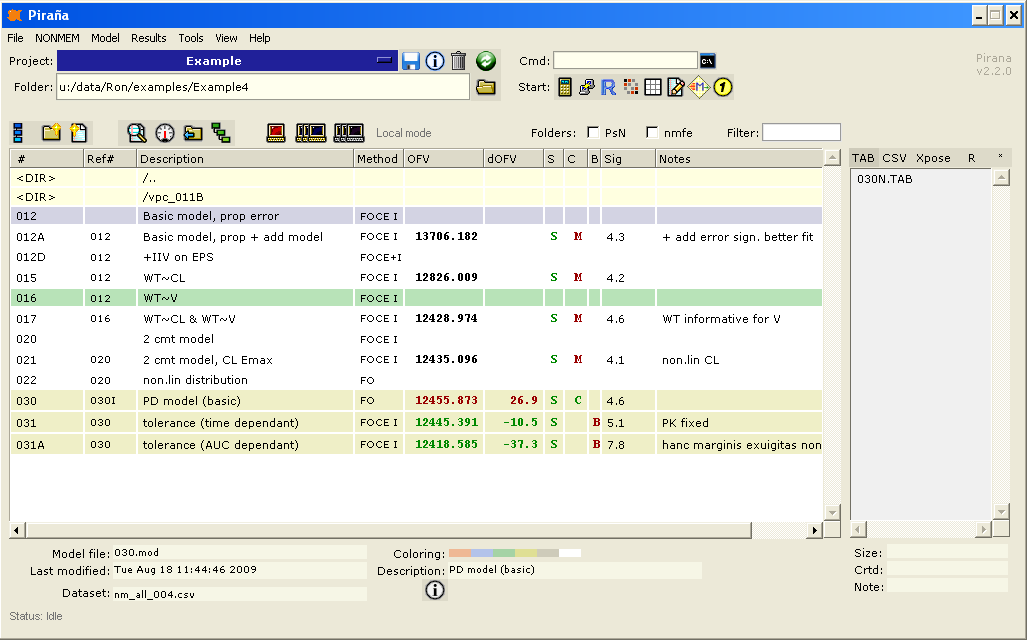
\includegraphics[scale=0.3]{images/main_screen_2.png}
    \caption{Pira\~na main screen}
\end{figure}

\subsubsection*{Model management} The main table is the place
where all models and subdirectories in the current working directory
are displayed. Only models are displayed that have a file-extension
corresponding to the file extension for model files specified in the
\textit{preferences}. When double-clicked, models are opened in the
code-editor (if specified), or else in Pira\~na's built-in NM-TRAN
editor. Models can be filtered using the `Filter' above the main
overview table. This filters all models based on the columns: run
number, description, and notes.\\

New models can be created from scratch, from a template, or by duplicating
an existing model. Some basic template models are included, but it is
possible to build your own library with base models that you often
use. Templates can be added by copying a model file to
\ttfamily{/templates }\normalfont in the Pira\~na directory. The
template models should have the same file extension as your model
files to be recognized as a template.

Duplication of models can be performed easily by selecting the parent
model and clicking `duplicate' from the context-menu (right click on the model).
Final parameter estimates from the reference model can be updated in the new model,
and also model-file numbers in \$TABLE and \$EST records. Some basic
syntax rules should be adhered to, see Conventions and Methods at the
end of this chapter.

\begin{figure}[hbt] \centering
    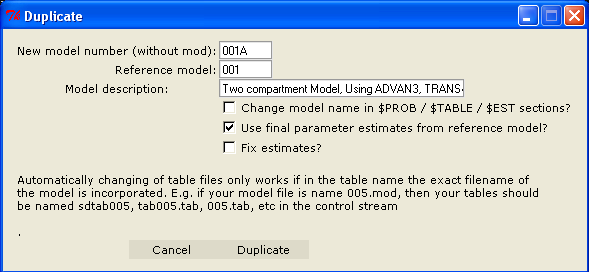
\includegraphics[scale=0.4]{images/duplicate.png}
    \caption{Duplicate model}
\end{figure}

\subsubsection*{Notes and colors}
Pira\~na offers the option to store notes about models in a
database. For this, in each active folder that is visited with
Pira\~na, a small SQLite database is created (`pirana.dir') which is
able to record model information. To add notes to a model, select the
model and click the model properties from the menu, or the `(i)' icon
from the dashboard on the bottom. Models and results can also be given
a color, which is done by selecting the model and clicking on the
desired color from the dashboard. The meaning of the color-coding is
of course all up to you!

\begin{figure}[hbt] \centering
    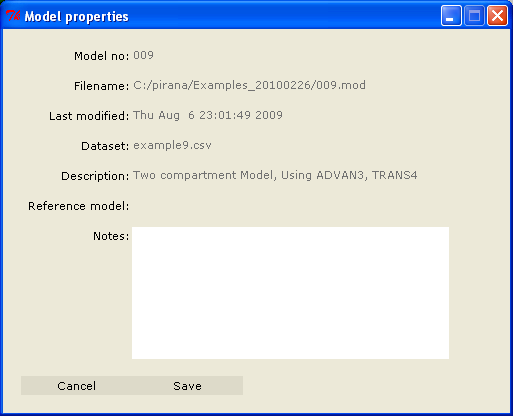
\includegraphics[scale=0.4]{images/model_properties.png}
    \caption{Model properties}
\end{figure}

\subsubsection*{Projects} Pira\~na can handle multiple projects, which are shown in the blue bar above the active folder entry, and
enables instant switching between them. To add a project to the list,
browse to a folder by clicking on the folder-icon next to the location
bar, or by clicking through the directory-listing in the model
overview. Next, click the `save'-icon next to the
`Project'-listbox, give your project a unique name and press the save
button. Your project is now available from the listbox. To delete
a project from the list, click the trash icon next to the project
list. The green refresh-icon refreshes the view of the current directory.

\subsubsection*{Data files} The right table shows the data-files, R
scripts, Xpose files, and other files, which are selected by clicking
the desired tab button above the box. The file extension of `tab' and
`csv' file-types can be set in the preferences while the XPose
filenames should adhere to the conventions specified in the XPose
manual (sdtab, patab etc). Right-clicking on a selected model shows
optional actions on the file.

\vspace{8pt}
\noindent\scriptsize{\textcolor{Blue}{Note:} \textcolor{Grey}{When the
XPose option is chosen, only unique run numbers are shown, instead of
all tabualar data files. When, after an XPose dataset is chosen, the
`X'-button is clicked, R will open with the selected dataset in XPose.
} \normalsize

\subsubsection*{Buttons: Models, runs, folders} Several buttons are
available from the Pira\~na main screen for changing the model
overview, or perform actions on models (left set of buttons). In the
middle set of buttons, functionality is included for e.g. viewing a
log of run executions, intermediate run results. On the right, two
checkboxes are implemented controlling the visibility of folders
created by Pira\~na and PsN. The `nmfe\_' folders are filtered out
from the Pira\~na model list by default, but these can be made visible
by checking the 'nmfe' checkbox, located above the model list. The
same is done for `modelfit\_' and `npcdir\_' directories created by PsN.}
\normalsize


\subsubsection*{Buttons: Quick links} Next to the active directory entry, a bar
with quick links to useful programs is shown. The location of these links
point to can be changed in `File $\rightarrow$ Software'.

\subsection*{Managing NONMEM installations} Existing NONMEM
installations can be added to Pira\~na using `Manage installations'
from the `NONMEM' menu. Here, both local and cluster (connected to through
SSH) installations can be added and made available in Pira\~na.

It may sometimes be necessary to increase (or decrease) internal
variable sizes, after which NONMEM has to be re-compiled. Pira\~na can
take care of this for you, but only for local regular (non-NMQual)
installations of NONMEM. In the `Manage NONMEM installations' dialog,
all settings found in the \ttfamily{SIZES} \normalfont file of the
active NONMEM installation can be edited and saved here, and the
installation can be re-compiled. The variables for NMQual NONMEM
installations can be viewed but not edited.

\subsection{Running models}
\subsubsection*{General}
When one or more NONMEM installations have been added to Pira\~na,
starting a model execution is easy: select a model from the list,
right-click to show the context-menu, and click `Run (nmfe)', or press
Control-R. This will open up a dialog showing two additional options
for running the model, e.g. which NONMEM installation to use, and if
models should be executed in separate folders or on a cluster system.

\subsubsection{Using PsN}
Models can also be run by one of the PsN-toolkit functions (execute:
Control-E, vpc: Control-V, bootstrap: Control-B, etc.). The procedure
is similar to described above, but now, a different dialog window is
opened (shown below), which also shows the PsN-help info for the
selected command.  The command line editor can be used to specify
additional specifications to PsN. Pira\~na stores the last command for
each of the toolkit functions, so you don't need to retype the bulk of
your command-line each time you use it.

\begin{figure}[hbt] \centering
    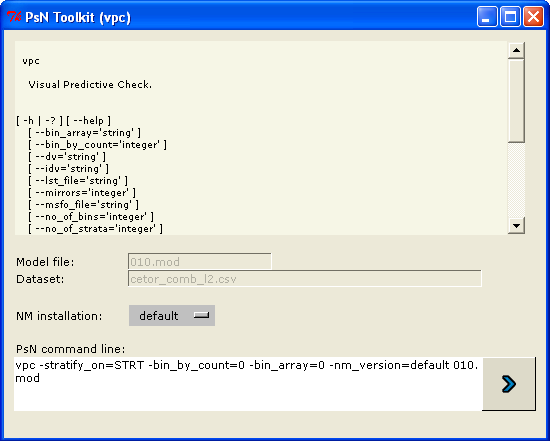
\includegraphics[scale=0.4]{images/psn_dialog.png}
    \caption{PsN dialog window}
\end{figure}

\subsubsection*{Using Wings for NONMEM} On Windows, Pira\~na is
capable of invoking the WFN-commands \emph{nmgo} and \emph{nmbs}, for
run execution and \emph{nmbs} for bootstrapping respectively. Since
WFN does not support multiple model files to be processed by its
commands, when multiple models are selected, only the first model file
is executed. When the WFN method is selected, two parameter
specification bars will become visible. In the upper entry, run
parameters can be specified, e.g. for the bootstrap: `1 100' to
specify a bootstrap with 100 replicates. The lower parameter bar
specifies command-line parameters used when starting WFN.bat,
e.g. `g77 std' for specifying the compiler and the NONMEM version to
be used. More information about WFN:
\textcolor{Grey}{http://wfn.sourceforge.net/wfninst.htm},
\textcolor{Grey}{http://wfn.sourceforge.net/wfnnmver.htm}.

\vspace{10pt}
\noindent\scriptsize{\textcolor{Blue}{Note:} \textcolor{Grey} {What Pira\~na actually does when executing runs through WFN, is create a temporary batch-file in the current directory that starts \emph{WFN.bat} to load the necessary environment variables, after which \emph{nmgo} is started with the model-file and parameters specified.}
  \normalsize

\subsection{Analyzing output}

\subsubsection*{HTML and \LaTeX \hspace{2pt} run reports} Run reports
can automatically be generated from NONMEM output of completed runs in
HTML or \LaTeX \hspace{2pt} format. The HTML output optionally
displays basic run information, run statistics, description and notes,
and parameter estimations for all estimation methods performed. The
information to be included in the report can be specified in the menu
under `Results $\rightarrow$ Include in run reports'. \LaTeX output is
opened in the specified code editor, but also can be converted
automatically to PDF, by setting the `pdflatex' setting to 1 in the
preferences.

\subsubsection*{Intermediate results} When running models through any
of the available methods, the intermediate results (parameter
estimates, objective function value (OFV), gradients) can be viewed by
clicking on the "gauge"-icon (lower left button from the results
buttons). This will open the window shown in the figure below, which
shows the models that are currently running. By Clicking on a run
intermediate data from INTER and OUTPUT files will be gather, and
returned in the table and the plot. Note that some Fortran
compilers (e.g. g77) do not support the real-time updating of these
output files, and that for such NONMEM installations, this function
will not work properly.

\begin{figure}[hbt] \centering
    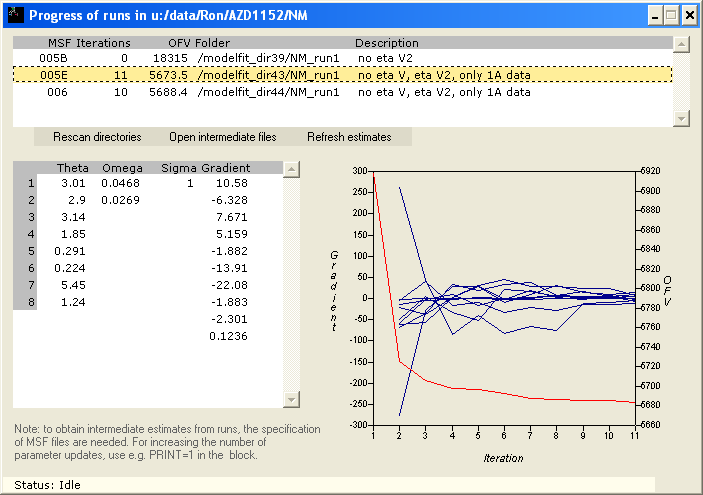
\includegraphics[scale=0.3]{images/intermed.png}
    \caption{Intermediate results}
\end{figure}

\subsubsection*{Plot functionality} Pira\~na is able to construct
scatter plots using the built-in 'Data-Inspector', e.g. for quickly
inspecting goodness-of-fit, covariate relationships, distribution of
etas, performing data checkout etc. The Data Inspector shows all the
columns present in the dataset, which can be plotted on the X- or
Y-axis (shown in figure 3.2).
\begin{figure}[hbt] \centering
    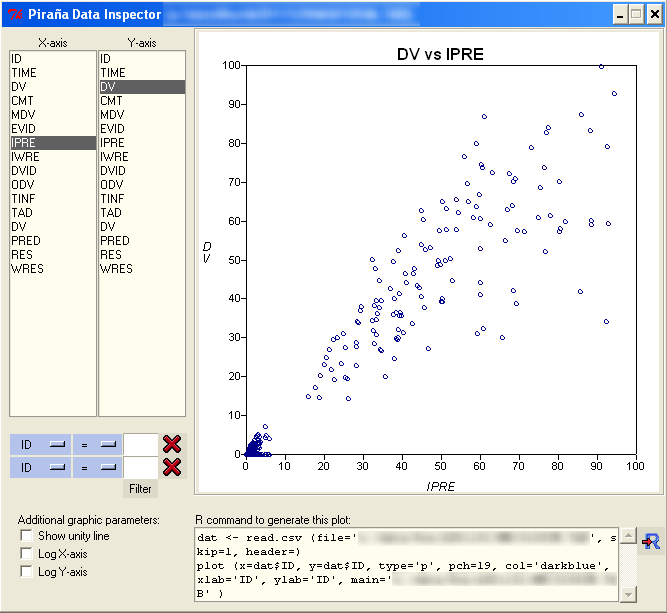
\includegraphics[scale=0.3]{images/plot.png}
    \caption{Pira\~na plot functionality}
\end{figure} Pira\~na can handle NONMEM-generated tables (either created with the
ONEHEADER and NOHEADER options), and CSV-files. Multiple Y values can
be plotted by holding the Control- or shift-key and selecting multiple
(up to three) data columns.

Inside the plot, regions of interest may be selected, which are
then zoomed. Double-clicking inside the plot region changes
back to the previous view. Plots can be filtered, which can be useful,
e.g. to show only data for one patient, or groups of patients or
covariates.

In the text-box below the plot, a command is generated that creates
the same graph in R, which can be used as a starting point for the
generation of plots for manuscripts or reports. On Windows, clicking the
`R'-button will invoke the RGUI and create the plot. On Linux,
clicking the icon will open the code in the specified code editor.

\subsection{Scripts}
Pira\~na includes functionality to run custom R-scripts on models, or
output from models-executions such as tables. This feature makes
Pira\~na a very flexible tool to manage and evaluate modeling results,
as custom scripts are easily created and adapted to suit specific
needs. Scripts can be written by the user, but a considerable
collection of scripts is also bundled with Pira\~na. Of course, these
scripts may be used as starting point for your own
implementations. The scripts are located in two locations, one for
group-wide scripts (in the scripts-folder in the location where
Pira\~na is installed), and one for user-scripts
(`home/user/.pirana/scripts' on Linux, `C:$\backslash$Documents and
Settings$\backslash$user$\backslash$Application
data$\backslash$Pirana$\backslash$Scripts' on Windows). The folder
structure underlying the scripts folder is maintained within the
scripts menu, and scripts can be edited either by editing them from
outside Pirana, or by choosing them from the `Edit' menu option.

Scripts can be started by selecting a model, and selecting the desired
script from the menu. What happens now, is that Pira\~na invokes R and
runs the script in the directory `pirana\_temp' underlying the active
folder.  However, before execution, Pira\~na inserts an R object which
specifies model and results information, e.g. as:

\begin{verbatim}
models <- list (
   "003" = list (
     "modelfile"       = "003.mod",
     "description"     = "PK model digoxin",
     "reference_model" = "002",
     "data_file"       = "nm_pk_001.csv",
     "output_file"     = "003.lst",
     "tables"          = c("003.TAB", "sdtab003")
   )
 )
\end{verbatim}

\vspace{15pt} \noindent To automatically load PDFs or images that are created by
R after execution of the script, include e.g. the following line in
the script:

\begin{verbatim}
#PIRANA model_output.pdf
\end{verbatim}

\noindent where model\_output.pdf is the file that you want Pira\~na
to load. This may either be a PDF, or a common image format such as
PNG, JPG, or GIF. Please have a look at the scripts included with
Pira\~na for examples of how to get the most out of this
functionality.


\subsection{Other tools}

\begin {description}
  \item{\textcolor{Grey}{Covariance calculator}} This opens the
built-in `Covariance Calculator', which can be used to re-calculate a
covariance to a correlation on the SD-scale. The formula for
correlation that is used is:

\vspace{10pt}
$ \rho_{i,j} = \frac{{\omega_{i,j}}^2 }{\omega_{i,i} \cdot \omega_{j,j} }
$
\vspace{10pt}

with $\rho$ specyfing the correlation between two elements (i,j) in a
matrix, and $\omega$ specifying elements of $\Omega$ or $\Sigma$.

  \item{\textcolor{Grey}{Checkout dataset}} This will create (and open)
an HTML-file which displays a selected dataset using separate colors for
different event-types. This will thus show the dataset in a slightly more
convenient format for manual inspection than in a spreadsheet. The
function needs an EVID column in the dataset to work properly.
\end{description}

\subsubsection*{Batch operations}
\begin{description}
	\item{\textcolor{Grey}{Replace block}} This function enables
you to replace a whole block of code in selected model files, e.g. the
\$DATA block if you want all model files to use a different data file,
or the \$THETA block if you want to use other initial estimates.
	\item{\textcolor{Grey}{Add code}} With this function, lines of
code can be added to the beginning or the end of selected models.
	\item{\textcolor{Grey}{Batch duplicate}} Creates multiple
duplicates of one model file, with (optionally) updated run/table
numbers and final parameter estimates.
	\item{\textcolor{Grey}{Random simulation seeds}} In all
selected models, the \$SIMULATION block will be updated with new
seeds.
\end{description}

\section{Conventions and Methods}
\subsubsection{Control stream conventions}
\begin{itemize}
\item Pira\~na reads the description of the model from the first line. The
words `\ttfamily{\$PROBLEM}' \normalfont or `\ttfamily{Model desc:}'
\normalfont are recognized.
\item If you want to use the hierarchy functionality for models, you
should specify the reference model in the first few lines of the model
file. Pira\~na is flexible and compatible with Census, and understands
e.g. the following syntaxes:

\begin{verbatim}
; Ref=001.mod
; Ref. model:001.mod
; Ref:001.mod
; Parent=001.mod
; Parent model:001.mod
; etc...
\end{verbatim}

\item Pira\~na reads the decriptions for model parameters from the
model file (and not from the output file). They need to be specified
after a semi-colon, e.g.

\begin{verbatim}
$THETA
(3, 5, 11) ; CL/F
(10, 50, 100) ; V/F
\end{verbatim}

To correctly read a covariance block, the covariance term needs to be
specified as `COV', e.g.

\begin{verbatim}
$OMEGA BLOCK(2)
0.1 ; IIV CL/F
0.05 ; COV CL~V
0.1 ; IIV V/F
\end{verbatim}

\item When models are to be executed in a separate directory, files
needed for compilation (e.g. additional Fortran routines in
.FOR files), are copied automatically by Pira\~na. These files should
be specified in the \ttfamily{OTHER} \normalfont and \ttfamily{CONTR}
\normalfont entries on the \ttfamily{\$DATA} \normalfont record. If
more additional files are needed, you can instruct Pira\~na to copy this
file by adding this line to your control stream:
\begin{verbatim}
; INCLUDE=file1_to_be_copied.ext,file2_to_be_copied.ext,etc
\end{verbatim}

Note that PsN has it's own functionality for doing this.

\item For duplicating runs with updated initial estimates from the
previous run, it is required to declare \$OMEGA and \$SIGMA blocks
only once, and not on every new line in the block, except when
specifying BLOCK structures. E.g.:

\begin{verbatim}
$OMEGA 0.1 ; KA
$OMEGA BLOCK(2)
0.1  ; IIV CL/F
0.05 ; COV CL~V
0.1  ; IIV V/F
$OMEGA
0.1 ; EMAX
0.1 ; V2
\end{verbatim}

\end{itemize}

\section{Troubleshooting}

Reported errors encountered with previous releases have been
fixed. Please report new bugs on the website
(http://code.google.com/p/pirana/issues/list). A FAQ is also
available on the website.


%%% CLUSTERS %%%%%%%%%%%%%%%%%%%%%%%%%%%%%%%%%%%%%%%%%%%%%%%%

\chapter{Pira\~na and clusters}

\section{Clusters} Pira\~na facilitates interaction with Linux-based
clusters on which NONMEM and/or PsN are installed, and both MOSIX
clusters and the Sun Grid Engine are supported. Basically, two options
are available for working with Pira\~na on such systems.  The first,
and recommended option is to install Pirana only on the cluster-server, and start
Pirana from the modeler's PC using SSH X-window tunneling. This has
the advantage of requiring only one central installation of Pirana for
the entire modeling group, and Pira\~na and other modeling software is
installed in a controllable environment. This option is also available
for users that want to work on Windows, by using XMing or Cygwin/X on
the local Windows PC.  The other method is to install Pira\~na on each
modeler's PC and to connect using Pirana's `SSH-connect' mode. This
may require a few additional client- and server-side
installations. For using this, you need to mount the cluster drive
with your data on your local PC (e.g. using sshfs on Linux or
ExpanDrive on Windows). Also you need to have ssh installed (OpenSSH
on Windows), of which some details are specified below.

Additionally, Pira\~na supports the construction of a simple
Windows-based clustering system (PCluster), which will be described in a
subsequent section. PCluster makes it easy to set up a cluster using
e.g. PCs of colleagues, and is easy to install on Windows systems. It
must be noted however, that this kind of setup is slightly inferior to the
clusters mentioned above in terms of stability and performance. Only
if no funds or no IT know-how is available to a modelling group do we
recommend using the PCluster.

\subsection{MOSIX and SGE}
While MOSIX systems distribute all active programs automatically, jobs
for the SGE must be submitted to the queue controller (using `qsub'),
which then distributes the job to a node. If you are using an SGE
cluster, you should therefore switch on the `Run using SGE' option in
the `NONMEM' menu section, or set it in the `Preferences
section'. Basically, what Pira\~na does is submit all models that are
run using the `nmfe'-method to the queue controller, instead of
executing the job directly. If you want to use SGE with the
PsN-toolkit, use `-run\_on\_sge'. Please consult the PsN-documentation
or its developers for more information.


\subsection{Method 1: X-window tunneling}

\subsubsection*{Xming}
If Pira\~na is installed on a Linux-cluster, and accessed from a
Windows client, you need to have an X-window system installed, which
will enable the display of the Pirana window locally on your PC. Such
a system is Xming, which can be obtained for free from
http://sourceforge.net/projects/xming/. After installation of Xming,
start the Xming X-window server.

\subsubsection*{Using the cluster}
If everything is set up correctly, and the X-window server is started,
Pira\~na on the cluster can be accessed through SSH, e.g. by using the
SSH client. Now, you should be able to see the Pira\~na main
window. If you get an error saying that the display cannot be started
on localhost, you may have to enable X-window forwarding in OpenSSH or in
PuTTY.

\subsection{Method 2: SSH-mode}

With this approach, Pira\~na is installed on the local PC. OpenSSH or
PuTTY needs to be installed as well, and a drive-letter must be
available on your local computer that enables access to your home
directory on the cluster. This can be setup e.g. using ExpanDrive to
connect to the cluster through SFTP. Alternatively, if, on the remote
cluster a Samba server is installed, a connection can be established
by giving the following command:

\vspace{6pt} \ttfamily{NET USE Z:
$\backslash$ $\backslash$server\_name$\backslash$user\_name
/user:user\_name /persistent:yes}\normalfont \vspace{6pt}

\noindent Both on Windows and Linux, you need to specify in the
preferences the mounted remote diskspace and the local location
(ssh\_mount\_cluster, ssh\_mount\_local), which is used by Pira\~na to
translate local paths to paths on the remote cluster.  If everything
is set up correctly, the `SSH-mode' should be enabled when running a
model. Models can then be run in a similar fashion as explained in the
section for running models locally.

\subsubsection*{OpenSSH} In this mode, Pira\~na needs passwordless
SSH-access to the cluster. In contrast to Linux, SSH is not available
on Windows by default, but this can be achieved by installing a
Windows version of OpenSSH (download from
http://sshwindows.sourceforge.net/) or PuTTY
(http://www.chiark.greenend.org.uk/\~ sgtatham/putty/). After
installation, ensure that you have an encryption key pair installed so
that the cluster won't ask you for a password everytime you perform an
action on the cluster, which is explained below.

\subsubsection*{Installing Public and private authentication keys}

Either on Windows or Linux, type in a shell/console window:

\vspace{6pt} \ttfamily{ssh-keygen -t rsa}\normalfont \vspace{6pt}

\noindent When asked for a passphrase, just press $<$Enter$>$.  Now a
public and a private key have been created in c:$\backslash$Documents
and Settings$\backslash$User Name$\backslash$.ssh
(Windows) or /home/username/.ssh (Linux).  In you home directory on
the cluster, if it doesn't exist already, create the folder `.ssh'. In
this folder, create the file `authorized\_keys' (no extension) and add
the contents of id\_rsa.pub to that file and save it. Now you should
be able to login without being asked for a password (type 'ssh
user\_name\@cluster\_name' in a console window, and you shouldn't be
asked for a password anymore. If SSH asks you if you want to accept
the cluster as valid host, accept). Keep your private key secret. In
the Pira\~na preferences, speficy the username to connect to the cluster
(ssh\_login).

\vspace{10pt}
\noindent\scriptsize{\textcolor{Blue}{Tip:} \textcolor{Grey} {Tip: if you experience delays (about 5 secs) when logging in to the
server by SSH, this may be caused by a reverse DNS lookup. You can
circumvent this by adding `useDNS no' to the file /etc/ssh/sshd\_config
on the server. Restart the ssh server for the changes to take effect:
sudo /etc/init.d/ssh restart}
\normalsize


\section{Sun Grid Engine}

Sun provides an open-source job scheduling agent for Linux, which
enables the distribution of NONMEM runs, or PsN-toolkit jobs over
computer clusters. Pira\~na supports the use of SGE, and also provides
some functionality for managing the cluster.

\subsection{Installation}
The reader is referred to the SGE manual for further information on
setting up the SGE. If the SGE is up and running, no additional steps
have to be taken to be able to use it. Some SGE settings can be
specified in the Pira\~na preferences, but these are likely to be
correct by default.

\subsection{Working with the SGE}
Submitting the execution of a model using nmfe to the SGE, can be done
by selecting the `Run on SGE' from the `Run model' dialog window. This
submits the model instead of starting it locally. If you want to use a
PsN-toolkit command on the SGE, specify -run\_on\_sge on the command
line.

Clicking the `cluster'-icon (right-most run-icon in the pirana main
screen), the SGE-monitor window is opened and will display an overview
of currently running jobs. From the tabs, also scheduled jobs, and
recently finished jobs can be viewed, and the nodes can be inspected.

\begin{figure}[hbt] \centering
    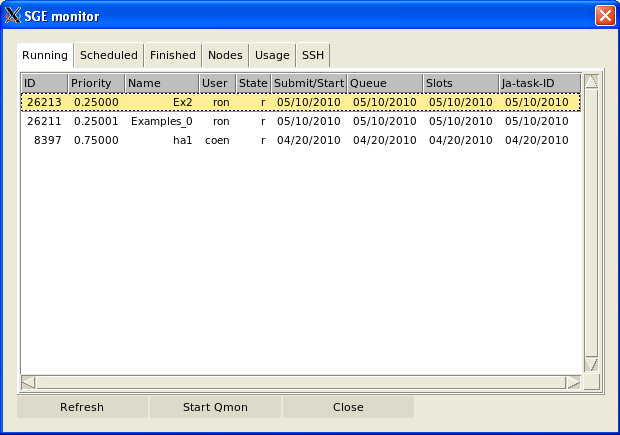
\includegraphics[scale=0.5]{images/sge_monitor.png}
    \caption{SGE monitor}
\end{figure}


\section{PCluster} The \textcolor{Blue}{PCluster} system is aimed to
be a system for distributed NONMEM computing for smaller modeling
groups, e.g. in hospital or academic settings. If budget poses no
problems, other cluster solutions are probably more adequate. Our major development goal
was to develop a system that could be installed on an existing
(Windows-based) network, and that would use spare CPU cycles of
non-dedicated PCs in the network.

\subsection{Description and requirements} The infrastructure uses
PC's in a standard Windows network environment, which can e.g. be PC's
dedicated to running NONMEM, or PC's of co-workers, or a combination
of both. The PCluster can be set up without the need for vast
hardware/software knowledge. Distribution to multi-core CPU's is
possible, and tested up to a total of 40 CPUs.

The infrastructure requires a shared network-drive accessible by all
clients (standard desktop PC's in a network environment). On this
shared network drive, a version of Perl and Fortran must be
present. Furthermore, the PCluster \textit{daemon} Perl-script
needs to run in the background on each node. On
the client computer, i.e. the modeler's computer, Pira\~na needs to be
installed. Below, more information is provided on how to set this up.

\subsection{Installation} First, it is necessary to reserve up some
harddisk space on your network, to be accessible (read and write) by
all clients, mounted as a drive on all nodes (let's assume this to be
U:). Copy the contents of the folder
\ttfamily{\/install\_on\_each\_node} \normalfont in the
\ttfamily{/cluster} \normalfont folder in the Pira\~na home folder to
this drive. Next, the daemon script (or the compiled version of it) should be
installed and running on each client in the network. For this, copy
the folder $\backslash$pcluster$\backslash$install\_on\_each\_node located in the Pirana home folder in the
harddisk root (C:$\backslash$). The daemon can be started manually by
executing the Perl script daemon.pl or the daemon.exe.  Before
starting, check the settings in
C:$\backslash$pcluster$\backslash$pcluster.ini. This file contains the
info for the client, e.g. the number of CPUs to use, and how to
connect to the shared drive.  Instead of starting the daemon manually, it is recommend to run the daemon as Windows service, which has the advantage that users are able to log in and out without compromising the integrity of the PCluster, and that
the service is automatically started when the PC is started. To
install this service, run the Perl script inst\_daemon.pl:
\begin{verbatim} perl inst_daemon.pl
\end{verbatim} This will create the information in the Windows
registry for the PDaemon service. If no error is reported, the service
can now be started from the command line with:
\begin{verbatim} NET START PDaemon
\end{verbatim}

It has been reported that the daemon sometimes isn't working properly
(i.e. not requesting PsN/nfme runs), while the script \'is working
properly when it is run manually. Running the daemon manually is
however a problem, as a console window will appear each time a run is
processing, which is annoying to the principal user of the machine. A
workaround for this is to download a tool called CMDOW (available from
http://www.commandline.co.uk/cmdow/). If you start the following
command (e.g. in a batch script at startup), no consoles will appear:
\begin{verbatim} u:\cmdow.exe /run /hid u:\perl\bin\perl.exe c:\pcluster\pdaemon.pl
\end{verbatim}

\vspace{8pt}
\noindent\scriptsize{\textcolor{Blue}{Note:} \textcolor{Grey}{Thanks
to Andreas Lindauer for suggesting this workaround.  } \normalsize


\subsubsection*{Perl and PsN} Make sure Perl (with
PsN installed) is available on the cluster-drive (e.g. in
U:$\backslash$Perl). Also check that you have the following Perl
modules installed: LockFile, Sys::Hostname and File.  Since this
option hasn't been fully developed yet in PsN, it is necessary to make
a few changes in some PsN source files (using PsN 3.1.0 as a
template).
\begin{itemize}
\item In \textcolor{Blue}{nonmem.pm} in the PsN directory, add the
following lines at the top of the source-file:
\begin{verbatim}
my $fortran_dir = 'U:\MinGW\bin';
unless ($ENV{'PATH'} =~ m/$fortran_dir/) {
  $ENV{'PATH'} = $fortran_dir.";".$ENV{'PATH'};
}
\end{verbatim} This ensures the Fortran compiler is in the path
(change U:$\backslash$MinGW$\backslash$bin' to the fortran path that
you use). Of course this is not necessary if this directory is
already permanently in the PATH environment variable.

\item In \textcolor{Blue}{tool$\backslash$modelfit.pm} change line
3014:
\begin{verbatim}
  require File::Temp; # qw/tempfile tempdir/;
  require Sys::Hostname;
  require LockFile::Simple; # qw/lock unlock trylock/; #Non-standard module
\end{verbatim}
into
\begin{verbatim}
  use File::Temp qw/tempfile tempdir/;
  use Sys::Hostname;
  use LockFile::Simple qw/lock unlock trylock/;  # Non-standard module
  use File::Basename;
\end{verbatim}

In the same file, move the contents of line 3063:
\begin{verbatim}
  return $jobId;
\end{verbatim}
to line 3057, just after the line with `unlock \$jobId;'.

In the same file, around line 3105, change:
\begin{verbatim}
  if( -e "$ZinkDoneDir$jobId" ){
\end{verbatim}
into
\begin{verbatim}
  use File::Basename;
  my $job = basename($jobId);
  if( -e "$ZinkDoneDir/$job" ){
\end{verbatim}

\item In psn.conf file in the PsN folder on the cluster, edit the
following lines with your settings (also remove leading semi-colons):
\begin{verbatim}
40 : perl = U:\Perl\bin\perl.exe
82 : zink_dir = U:
105: default=U:\nmvi,6
\end{verbatim} Of course, the other PsN settings should be set correctly as well.

\end{itemize}

\subsubsection*{Fortran (g77)} If you want to use the PsN-toolkit on
the PCluster, you must provide access to a Fortran compiler for each
client in the cluster. This is because PsN runs are compiled after
distribution to a client. If you only make use of Pirana's own
distribution capabilities, only a Fortran compiler on the modeler's
own computer is required. The recommended way is to use a central
installation of Fortran on the cluster drive, e.g. g77 supplied with
MinGW. For this, e.g. install MinGW with g77 on your local
computer. After installation, copy the folder MinGW to the cluster
drive.

\subsubsection*{Pirana preferences} In Pira\~na the following
preferences should be updated:
\begin{description}
	\item \textcolor{Grey}{zink\_host}:
e.g. \textcolor{Blue}{ZinkHost}, A host name for the Zink / PCluster,
should correspond with the hostname specified in psn.conf.
\end{description}
\noindent And in `software settings', change:
\begin{description}
  \item \textcolor{Grey}{f77\_dir}: Path to Fortran on the
cluster-drive e.g.  \textcolor{Blue}{U:/MinGW/bin}
  \item \textcolor{Grey}{perl\_dir}: Path to Perl on the cluster-drive
e.g.  \textcolor{Blue}{U:/Perl}
  \item \textcolor{Grey}{psn\_dir}: Path to PsN on the cluster-drive
e.g.  \textcolor{Blue}{U:/Perl/site/lib/PsN\_2\_3\_1}
\end{description}

\subsubsection*{Troubleshooting} The PCluster, although it functions
quite adequately in the current setup, is actually still in beta
phase. If you have questions regarding the set-up or functionality of
the PCluster, please send a mail to the mailinglist
(\textcolor{Grey}{pirana-users@lists.sourceforge.net}) or contact the
Pira\~na development team directly.

\pagebreak
\subsection{Working with the PCluster}

\subsubsection*{Using the PsN toolkit on PCluster} This functionality
is enabled by specifying `-run\_on\_zink' on the PsN command line from
the Pira\~na window, after selecting a PsN tool from the toolkit. You
should leave the PsN console window open until the run is finished,
since the instance of PsN that is running locally will take care of
the run distribution and calculation and formatting of data files
after finishing the cluster run(s).

\subsubsection*{Cluster monitor} Using the cluster monitor (`View
$\rightarrow$ Cluster monitor') the activity and availability of
clients can be monitored. Note that status of the client might take a
half a minute to refresh with the up-to-date information, due to the
interval used by the daemon-script.  \vspace{10pt}

\begin{figure}[hbt] \centering
    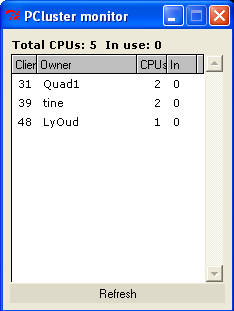
\includegraphics[scale=0.5]{images/pcluster.png}
    \caption{PCluster monitor}
\end{figure}

\chapter{Endnotes}
\section{Acknowledgements} For testing and feedback, thanks to
(ex-)colleagues in the modeling \& simulation group of the Slotervaart
Hospital / the Netherlands Cancer Institute. Also various modelers
from around the world are recognized for their valuable suggestions
and bug-reports. The Uppsala PM group for good ideas and
providing their Mosix-cluster for testing.

\section{Disclaimer} This software is provided as free software under
an open source license (GNU General Public License) and on an `as is'
basis, without warranty of any kind. Your use of the software is at
your sole risk, and the author cannot be held liable for any harm,
inflicted upon your system by this program.\\ \vspace{5pt} \\
Questions, comments, tips or bug-reports are very welcome at the the
bug report list (http://code.google.com/p/pirana/issues/list), or at
the mailinglist
(http://pirana.sourceforge.net/mailinglist.php). Please be as specific
as you can about the issue. Also, if you would like to contribute to
the development of Pira\~na, please contact us.

\section{Aims for future versions}
Currently we are working on a quality assurance system for Pira\~na,
which is already partially in place. Documentation will be posted
online when available.

\subsubsection*{Aims for version 2.4.0: January 2011?}
\begin{itemize} \scriptsize
  \item Support for parallel NONMEM
  \item Enhance reporting features
\end{itemize}

\section{Version history}
\subsubsection*{Updates for version 2.3.0 (\textcolor{Grey}{"Oahu"}):
April 2010}
\begin{itemize} \scriptsize
  \item NONMEM 7 output support
  \item Added scripts functionality
  \item Added SGE support
  \item Improved Linux support
  \item Included NM help, improved PsN help
  \item Updated manual and website
\end{itemize}

\subsubsection*{Updates in version 2.2.0
(\textcolor{Grey}{"Pipeline"}): November 2009}
\begin{itemize} \scriptsize
  \item Linux / Mac OS X compatible
  \item Multi-user functionality
  \item Basic NONMEM 7 support
  \item Much improvements to GUI
  \item bug-fixes
\end{itemize}

\subsubsection*{Updates in version 2.1.0 (\textcolor{Grey}{"Waimea
Bay"}): August 2009}
\begin{itemize} \scriptsize
  \item Full screen mode
  \item Plots of gradients and OFV in intermediate results window
  \item Keep log of model executions
  \item More functionality for documenting models, tables and
projects.
  \item More structure and documentation in source code
  \item Changes to GUI and Bugfixes
\end{itemize}

\subsubsection*{Updates in version 2.0.1
(\textcolor{Grey}{"Hookipa"}): May 2009}
\begin{itemize} \scriptsize
  \item Added $\delta$ OVF in model overview
  \item Resizable column headers in model overview
  \item Added minimization text to HTML output
  \item Overlay multiple Y-columns in Data Inspector plot (hold
ctrl-key)
  \item Improved NONMEM run options in GUI
  \item Improved adding of NONMEM installations, NMQual/regular
installations detected automatically
  \item Automatically detect PsN NONMEM installations
  \item Added covariance calculator
  \item Added dataset checkout function
  \item Bug-fixes
\end{itemize}
\subsubsection*{Updates in version 2.0.0
(\textcolor{Grey}{"Waikiki"}): March 2009}
\begin{itemize} \scriptsize
  \item Changed GUI: models and results in one window. More
notebook-like, add notes and highlighting.
  \item Access linux-based (Mosix) clusters through OpenSSH. Use nmfe
and PsN-toolkit on these clusters.
  \item Added support for running PsN toolkit on PCluster
  \item Overview of active runs in (sub)folders, show intermediate
results and gradients.
  \item Removed reliance on PsN for creation of summary of run result.
  \item Quick view of parameter estimates window
  \item Create csv summary of all models and results
  \item Added filters to Data Inspector
  \item Added Installer
  \item Lots of bug-fixes
\end{itemize}
\subsubsection*{Updates in version 1.3: September 2008 (not released)}
\begin{itemize} \scriptsize
  \item Replaced R-plots with general plotting functionality (Data
Inspector)
\end{itemize}
\subsubsection*{Updates in version 1.2.1: August 2008}
\begin{itemize} \scriptsize
  \item Added more WFN support: custom compiler / NM version
\end{itemize}
\subsubsection*{Updates in version 1.2: June 2008}
\begin{itemize} \scriptsize
  \item Fixed the script for bootstrapping on the PCluster
	\item Added feature: Run models using NMQual NONMEM
installations
	\item Added feature: Install NONMEM from NMQual XML files
	\item Added feature: Support for Wings for NONMEM (nmgo/nmbs)
	\item Added new functions for monitoring cluster runs
\end{itemize}
\subsubsection*{Release version 1.0: May 2008}
\begin{itemize} \scriptsize
  \item First release version
\end{itemize}

\end{document}
